\documentclass{report}

\usepackage{graphicx}
\usepackage{float}
\usepackage{wrapfig}
\usepackage{color}
\usepackage{siunitx}
\usepackage[usenames,dvipsnames]{xcolor}
\usepackage[english]{babel}
\usepackage{amssymb}
\usepackage{geometry}

\begin{document}

\title{\textbf{Homework 5:} $\mathcal{A}x=b$: Solving systems of linear equations using Gauss-Jordan and LU decomposition}
\author{A.L. Phillips II\\
  Department of Physics, Astronomy, and Applied Physics,\\
  Rensselaer Polytechnic Institute\\
  \texttt{philla3@rpi.edu}}
 \date{26 April 2013}
 \renewcommand{\chaptername}{Assignment}
 \setcounter {chapter}{4}
\maketitle

\chapter{System of Linear Equations}

\section{Gauss-Jordan Elimination}
\begin{enumerate}

\item Runge-Kutta (RK) is a numerical method which allows for the approximation of solutions to systems of ODE's.  There are several versions of the method which vary with order $N$. Here, RK4, also known as Classical-RK, will be discussed. 
\\
\\For a given set of required initial conditions, RK4 approximates $ y_{n+1} $ at a later time $ t_n+h$, where h is a chosen time step size. The method makes use of a weighted average of approximated values and is given by the following:
\\
\begin{eqnarray*}
\ y_{n+1}&=&y_n+\frac{h}{6}(k_1+2k_2+2k_3+k_4)\\
\\\
\ k_1 &=& f(t_n,y_n)\\
\ k_2 &=& f(t_n+\frac{h}{2}, y_n+\frac{hk_1}{2})\\
\ k_3 &=& f(t_n+\frac{h}{2}, y_n+\frac{hk_2}{2}) \\
\ k_4 &=& f(t_n+h, y_n+hk_3) \\ \\
\end{eqnarray*}

\end{enumerate}



\section{Resistor Arrays}
\begin{enumerate}
\item 
\begin{figure}[H]
\centering \caption{5 x 3 Resistor Array. 1$v$ Source, 1$\Omega$ Resistors}
\includegraphics[scale=.92]{sej.eps}
\label{sej}
\end{figure}
\\
\\In simple circuits, solving for equivalent resistance, voltage and current across series and parallel devices is done using $\displaystyle V=iR$. To find the equivalent resistance of the entire circuit, find the resistance "felt" by the voltage source. 
\\
\\This is done by dividing the Voltage by the current through the voltage source: 
\begin{center}
$\displaystyle R_{equiv}=\frac{V}{i}$. 
\end{center}
The equivalent resistance between individual devices may be found through direct or reciprocal addition. For resistors in series, the resistances between devices increases, therefore: 
\begin{center}
$\displaystyle R_{equiv} = R_1 + R_2$ (Resistors in Series)
\end{center}
For resistors in parallel, the resistance is less then the smallest resistance of the devices in parallel, therefore:  
\begin{center}
$\displaystyle R_{equiv}=\frac{1}{R_1} + \frac{1}{R_2}$ (Resistors in Parallel)
\end{center}
In the case of a resistor array such as that depicted below, the task of solving for these concepts may become tedious through daunting. To simplify the problem, Kirchhoff's loop rule is implemented in order to devise a matrix of resistances and a vector of currents and voltage. 

\[ \left( \begin{array}{ccccccccccccc}
3&-1&0&0&0&-1&0&0&0&-1&0&0&0 \\
-1&4&-1&0&0&-1&0&0&0&0&0&0&0 \\
0&-1&4&-1&0&0&-1&0&0&0&0&0&0 \\
0&0&-1&4&-1&0&0&-1&0&0&0&0&0 \\
0&0&0&-1&4&0&0&0&-1&0&0&0&0 \\
-1&-1&0&0&0&4&-1&0&0&-1&0&0&0 \\
0&0&-1&0&0&-1&4&-1&0&0&-1&0&0 \\
0&0&0&-1&0&0&-1&4&-1&0&0&-1&0 \\
0&0&0&0&-1&0&0&-1&4&0&0&0&-1 \\
-1&0&0&0&0&-1&0&0&0&4&-1&0&0 \\
0&0&0&0&0&0&-1&0&0&-1&4&-1&0 \\
0&0&0&0&0&0&0&-1&0&0&-1&4&-1 \\
0&0&0&0&0&0&0&0&-1&0&0&-1&4 \end{array} \right)\] 


t's equivale as shown below cant be daunting from the usual sense. Normally, into itThe motion of the planets may be described via Newtonian mechanics. We obtain the ODE's describing the acceleration from one body acting upon another as $\displaystyle F = ma = \frac{GMm}{r^2}$
Here $G$ is the Gravitational constant (\SI{6.67398e-11}), $M$ is the mass of the Sun, $m$ is the mass of the planet being acted upon and $r$ is the distance between the bodies. Decomposing $F$ into its components yields:
\begin{center}
$\displaystyle F_x = ma_x = \frac{GMm}{r^2}cos\theta = \frac{GMm}{r^2}\frac{x}{r} = \frac{GMmx}{r^3}$
\end{center}

\begin{center}
$\displaystyle F_y = ma_y = \frac{GMm}{r^2}sin\theta = \frac{GMm}{r^2}\frac{y}{r} = \frac{GMmy}{r^3}$
\end{center}

Since we are interested in obtaining a $2^{nd}$ order ODE ($\displaystyle \frac{d^2s}{dt^2}$) to model the motion of a planet, we will isolate the acceleration in the Force equations by dividing out $m$:  $\displaystyle \frac{F}{m} = \frac{ma}{m} = a$


Therefore, the two $2^{nd}$ order ODE's that we seek are:
\begin{center}
$\displaystyle a_x = \frac{d^2x}{dt^2} = \ddot{x} = \frac{GMx}{r^3}$
\end{center}
\begin{center}
$\displaystyle a_y = \frac{d^2y}{dt^2} = \ddot{y} = \frac{GMy}{r^3}$ 
\end{center}
In order to make use of our $2^{nd}$ order ODE's via RK4, we must reduce them to a simultaneous system of $1^{st}$ order equations via the following substitutions:
\begin{eqnarray*}
\ Let \quad z_x & = & \dot{x} \qquad \qquad (dydx[0] \; from \; NR3's \; rk4)\\
\dot{z_x} & = & \ddot{x} \qquad \qquad (dydx[1]  \; from \; NR3's \; rk4)\\
\ Let \quad z_y& = & \dot{y} \qquad \qquad (dydx[2] \; from \; NR3's \; rk4)\\
\dot{z_y} & = & \ddot{y} \qquad \qquad (dydx[3] \; from \; NR3's \; rk4)
\end{eqnarray*}
Initial conditions must be provided in order to make use of RK4's numerical solutions:
\begin{eqnarray*}
\ x(0) & = & x_0 \qquad \qquad (y[0] \; from \; NR3's \; rk4)\\
\ V_{x}(0) & = & V_{x}(x_0)\qquad (y[1]  \; from \; NR3's \; rk4)\\
\ y(0) & = & y_0 \qquad \qquad (y[2] \; from \; NR3's \; rk4)\\
\ V_{y}(0) & = & V_{y}(y_0) \qquad (y[3] \; from \; NR3's \; rk4)
\end{eqnarray*}
$.\qquad$ To avoid accumulating error with large step sizes, a small step size must be used. If, for example, we use $h=0.1 seconds$ for a time step size, we would have to set $k_{max}=315,360,000$ in order to calculate a full Earth orbit. Despite our step size being small, errors would still accumulate over the large number of iterations specified in $k_{max}$. A large $k_{max}$, while resulting in a higher sample rate, will also require longer execution time. To minimize error and time spent waiting for code completion, we may convert the problem and all its dependent constants (e.g. $G$) to astronomical units ($1AU=149,597,871 km$) and days. Making use of these larger units will now allow us to calculate a full earth orbit using $h=0.1 days$ over $ k_{max}=3650$ iterations.
\\
\\
\item The Sun, Earth and Jupiter:
\\
\\Modeling the orbits of Earth and Jupiter due soley to solar interactions produces the following plot. Note that the Sun is at the origin of all proceeding graphics:
\begin{figure}[H]
\centering \caption{\textcolor{red}{Earth} and \textcolor{blue}{Jupiter} about the Sun (non-interacting)}
\includegraphics[scale=.92]{sej.eps}
\label{sej}
\end{figure}
Notice that in the above plot, even though the eccentricity of the ellipse is exaggerated due to the differing scales used in the axes, it is still a strain to notice the difference between perihelion's and aphelion's. Using equal aspect ratios in the axes, shown below is a more accurate representation of the actual shape of the orbits. Ensure you are not seduced into thinking they are circular orbits; despite the small the difference, the major and minor axis are not equal.
\begin{figure}[H]
\centering \caption{\textcolor{red}{Earth} and \textcolor{blue}{Jupiter} about the Sun (non-interacting)}
\includegraphics[scale=.63]{sejCircle.eps}
\label{sejCircle}
\end{figure}
In addition, enabling the interactions that Jupiter and Earth have upon on each other yields the following plot:
\begin{figure}[H]
\centering \caption{\textcolor{red}{Earth} and \textcolor{blue}{Jupiter} about the Sun (interacting)}
\includegraphics[scale=.63]{sejCircle.eps}
\label{sej}
\end{figure}
While the effects of the planetary interactions are not apparent on a plot of this scale, zooming in upon the perihelion's of both Earth and Jupiter elicits further detail:
\begin{figure}[H]
\centering \caption{Orbits of Earth with Jupiter \textcolor{magenta}{Interaction} and Jupiter \textcolor{blue}{Non-interaction} at Perihelion}
\includegraphics[scale=.9]{interactEarth.eps}
\label{interactEarth}
\end{figure}
\begin{figure}[H]
\centering \caption{Orbits of Jupiter with Earth \textcolor{magenta}{Interaction} and Earth \textcolor{blue}{Non-interaction} at Perihelion}
\includegraphics[scale=.9]{interactJupiter.eps}
\label{interactJupiter}
\end{figure}

Notice that in the interaction plots above, Earth's orbit is greatly affected by Jupiter, whereas Jupiter's orbit is barely affected by Earth. Jupiter is the most massive planet in our solar system. It has over 300 times the mass of Earth and so these plots appear intuitive. As we have determined, $\displaystyle a = \frac{GM}{r^2}$, therefore the acceleration due to a body is directly proportional to its mass.
\\
\\
\item Kepler's $2^{nd}$ Law 
\\
\\$. \qquad$ Kepler's second law of planetary motion states that a line joining the Sun and a planet sweeps out equal areas in equal time intervals. 
\\
\\To show this, we will begin with the $\theta$-component of the Force from the Sun acting on a planet as follows:
\begin{center}

$F_\theta=m(r\frac{d^2\theta}{dt^2}+2\frac{dr}{d\theta}\frac{d\theta}{dt})$

\end{center}

We know that force exerted by the Sun on a planet is exclusively in the radial direction between the two bodies and so there is no $\theta$-component of $F_\theta$. 

Therefore, \begin{center}
$F_\theta=0=m(r\frac{d^2\theta}{dt^2}+2\frac{dr}{d\theta}\frac{d\theta}{dt})$

\end{center}
Dividing out mass and multiplying by r yields:

\begin{center} $0=(r^2\frac{d^2\theta}{dt^2}+2r\frac{dr}{d\theta}\frac{d\theta}{dt})$ \end{center}

Notice that by introducing r in the previous step, we expose the result of a product rule. The above may then be rewritten as a time differential as follows: 

\begin{center}$0=(r^2\frac{d^2\theta}{dt^2}+2r\frac{dr}{d\theta}\frac{d\theta}{dt})=\frac{d}{dt}(r^2\frac{d\theta}{dt})$\end{center} 

Integrating the $RHS$ of the above expression with respect to time yields the following:

\begin{center}$\int0 dt=\int[\frac{d}{dt}(r^2\frac{d\theta}{dt}]dt$\end{center}

\begin{center}$C=r^2\frac{d\theta}{dt}$ which may also be written as  $Cdt=r^2d\theta$\end{center}

Now, we know that the Area of an arc is give by $A = \frac{1}{2}r^2\theta$ and since we are looking for the area swept out by a planet, let $dA=\frac{1}{2}r^2d\theta$. Notice that since $Cdt=r^2d\theta$, then we may make the following substitution:

\begin{center}$dA=\frac{1}{2}(r^2d\theta) = \frac{1}{2}(Cdt)$.\end{center}

\begin{center}$\displaystyle \int^{t_2}_{t_1}dA =\int^{t_2}_{t_1} \frac{1}{2}Cdt$\end{center}

\begin{center}$\displaystyle A(t_2)-A(t_1)= \frac{C}{2}\int^{t_2}_{t_1}dt=\frac{C}{2}(t_2-t_1)$ \end{center}

\begin{center}Therefore, $A_{total}=A(t_2)-A(t_1)=\frac{C}{2}(t_2-t_1). \;$ 
\end{center}

Using the arc length formula, $rd\theta = ds$, allows us to rewrite our expression for $C$ as follows:

\begin{center}$C = r^2\frac{d\theta}{dt} = r(r\frac{d\theta}{dt}) = r(\frac{ds}{dt}) = rv$.
\end{center}
Plugging $C=rv$ into our expression yields $\displaystyle A_{total}=A(t_2)-A(t_1)=\frac{C}{2}(t_2-t_1) = \frac{rv}{2}(t_2-t_1)$.
\\
Here we see that for separate time intervals whose differences are equal, the Area swept out will be proportional to $rv$. Since $r$ increases as $v$ decrease and vice versa, the expression appears intuitive. 
\\
\\To verify this law numerically, the area swept out may be approximated by calculating the area of a triangle with vertices at the sun, position($t_{0}$) and position($t_{1}$). While this method (depicted below) appears to be a poor approximation of area, it is both easily implemented and improved by using smaller time intervals such that the area excluded is minimized.  
\begin{figure}[H]
\centering \caption{Approximating Kepler's $2^{nd}$ Law }
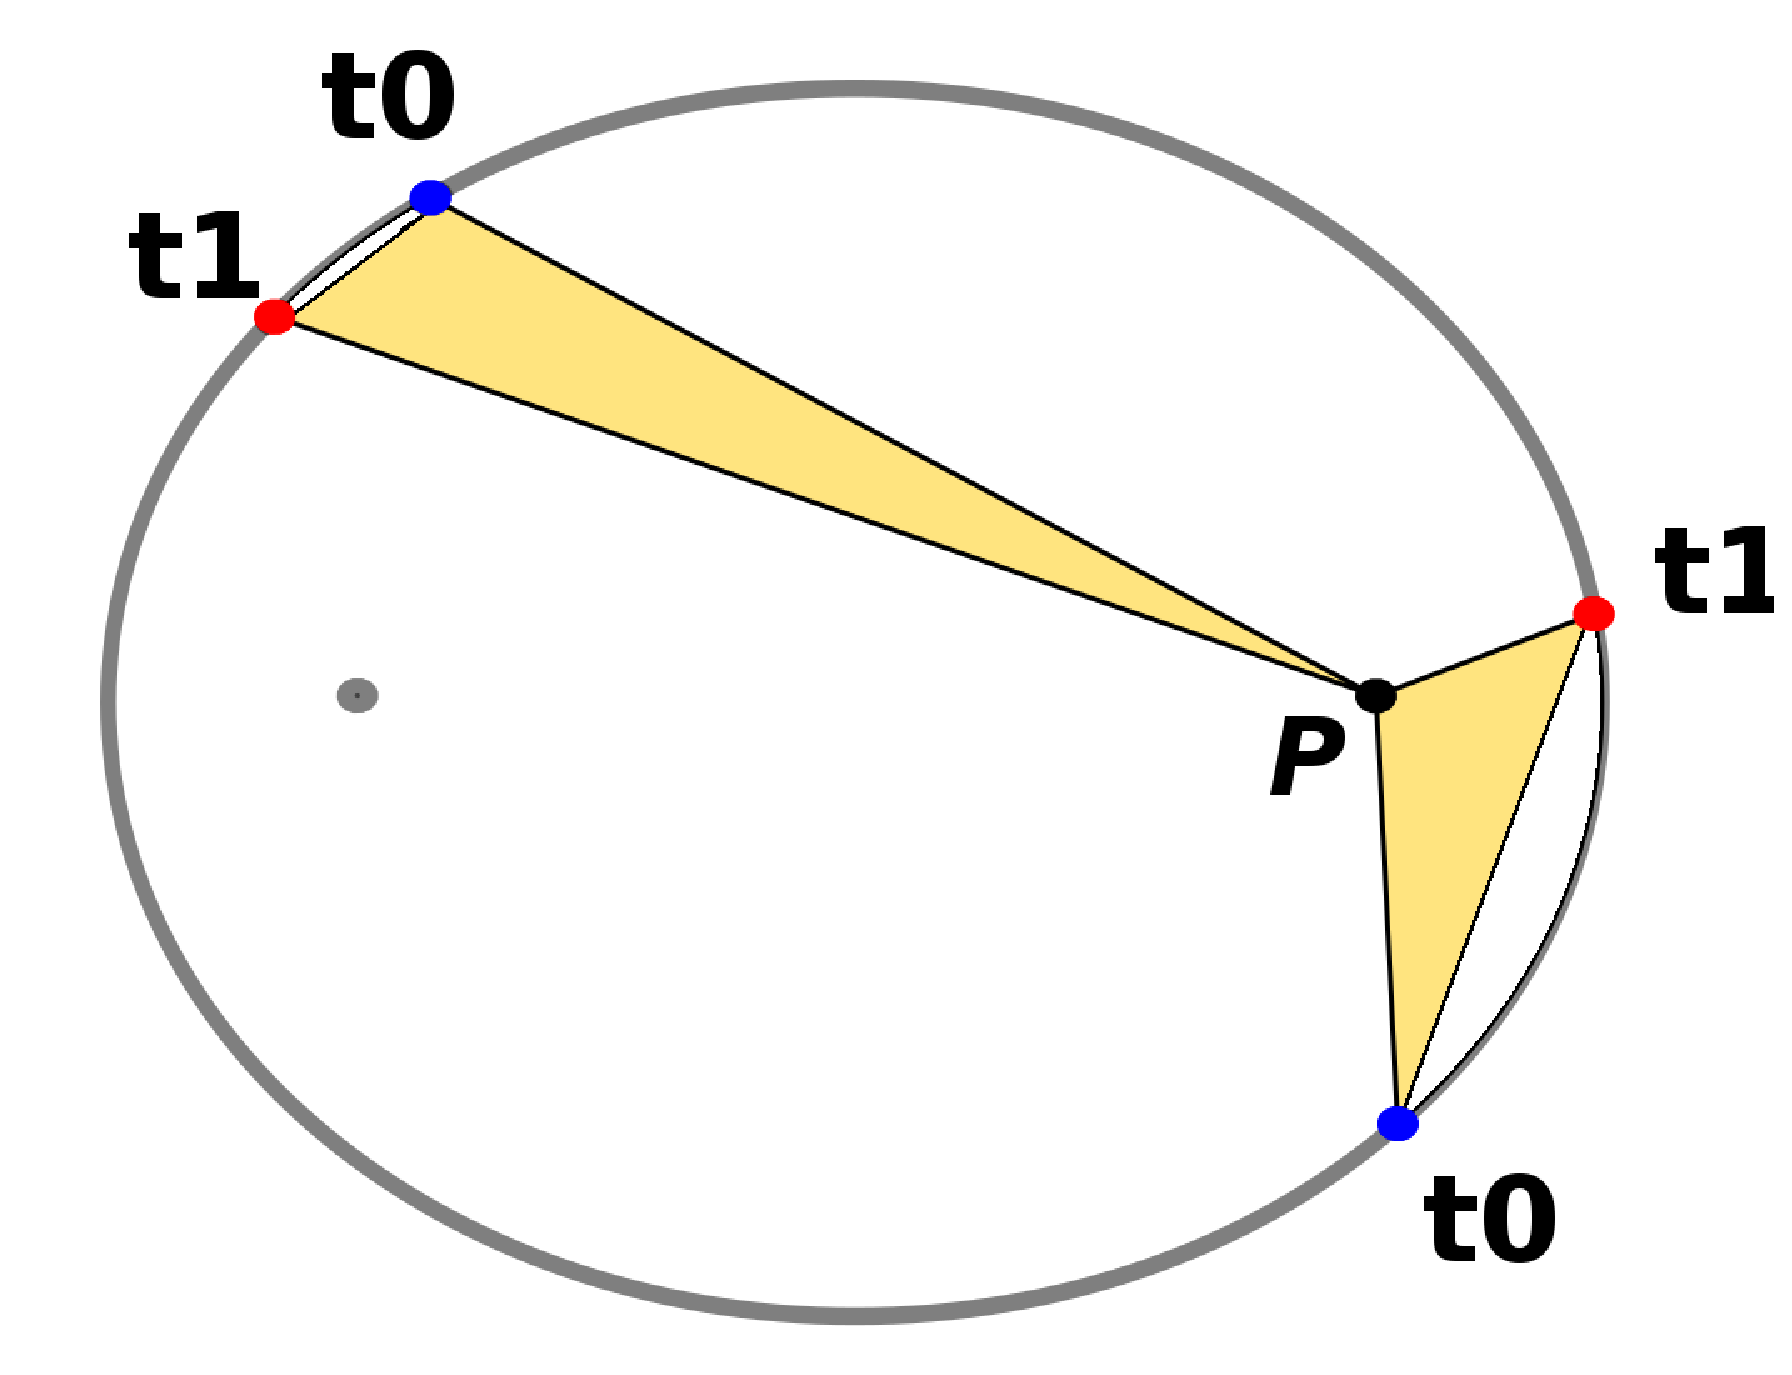
\includegraphics[scale=.25]{keplers2nd.eps}
\label{keplers2nd}
\end{figure}

\begin{center}
$\displaystyle Area_{\small (1^{st}week)} \approx \frac{\left|ad-bc\right|}{2} \approx \frac{\left|(0.98329)(0.113462)-(0)(0.97683) \right|}{2} \approx 5.57828e^{-2}$
\end{center}
$\displaystyle Area_{\small (25^{th}week)} \approx \frac{\left|ad-bc\right|}{2} \approx \frac{\left|(-0.990248)(0.119453)-(0.227742)(-1.00937) \right|}{2} \approx 5.57943e^{-2}$
\begin{center}
$\displaystyle \epsilon_{\small absolute} = \left| 5.57828e^{-2} - 5.57943e^{-2}\right| * 100 \approx 0.00115\%$
\end{center}
\item Fat Jupiter
\\
\\The effect on Earth's orbit of artificially increasing the mass of Jupiter is considerable. Jupiter's actual mass is approximately \SI{1.899e27} kg. Scaling this by a factor of $10^3$ brings the mass of Jupiter within 4.5\% of the Sun's mass. This would appear as a pseudo binary start system.
\\
\\We know that acceleration due to a body is expressed as $\displaystyle a = \frac{GM}{r^2}$. Therefore, even with Jupiter increased mass, the acceleration it exerts upon Earth must go as $\displaystyle \frac{1}{r^2}$. At the smallest radius between Jupiter Radius ($\approx 4$ AU's), the sun will still continue to exert an acceleration 17 times greater than Jupiter. At Jupiter and Earth's further radius ($\approx 6$ AU's), the Sun exerts an acceleration $\approx$34 times greater. In the proceeding result, both Earth and Jupiter were initially located at Perihelion with maximum velocities. This is of significance as different initial conditions may yield different results. 
\begin{figure}[H]
\centering \caption{Earth's orbit affected by Jupiter's \textcolor{Red}{Actual-Mass} and \textcolor{blue}{$10^3$Mass}}
\includegraphics[scale=.75]{fatEarth.eps}
\label{fatEarth}
\end{figure}
.
\item Precession of Mercury's Perihelion:
\\

Using the equation of Force modified with general relativity (GR) corrections to obtain the acceleration of the Sun upon Mercury yields: $\displaystyle a_{GR} = \frac{GM}{r^2}(1+\frac{\alpha}{r^2})$ where $\alpha$ is a small coefficient due to GR corrections.
\\
\\
\\Plotting the orbit of Mercury for $\alpha=0.008$ results in the following:
\\
\begin{figure}[H]
\centering \caption{Precession of Mercuries Perihelion}
\includegraphics[scale=.75]{precession.eps}
\label{fatEarth}
\end{figure}
.
\\
\\
\\
\\
\item The Double Pendulum
\\
\\\begin{figure}[H]
\centering \caption{A Double Pendulum}
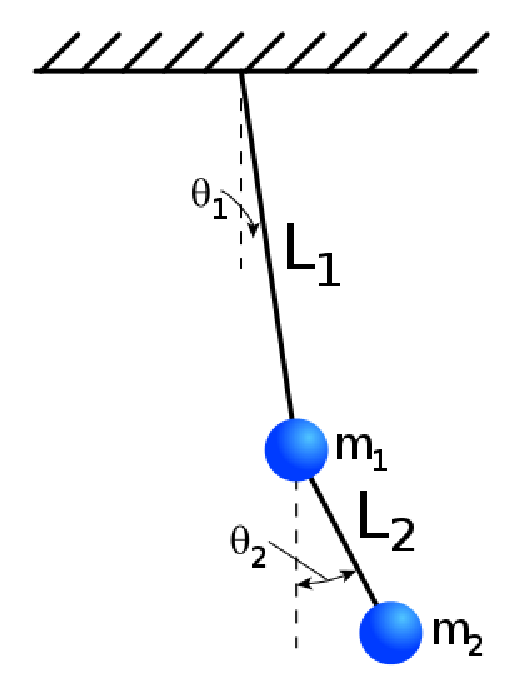
\includegraphics[scale=.8]{doublepend.eps}
\label{fatEarth}
\end{figure}
Shown above is the double pendulum. The coupled $2^{nd}$ order ODE's needed to model the motion of $m_1$ and $m_2$ may be obtained with Newtonian mechanics or conservation of energy via Lagrange/Euler methods. As I'm yet familiar with Lagrange/Euler methods needed to obtain the ODEs, I will take the tedious Newtonian route for derivation:
\\
\\To make a start, we begin with $F=ma$ and decompose the forces of each mass into their x and y components:
\\\begin{eqnarray*}
\ m_1\ddot{x_1} &=& F_{T2}sin(\theta_2)-F_{T1}sin(\theta_1) \qquad Mass_1 \; components\\
\ m_1\ddot{y_1} &=& F_{T1}cos(\theta_1)-F_{T2}cos(\theta_2)-m_1g\\
\ \\
\ m_2\ddot{x_1} & = & -F_{T2}sin(\theta_2) \qquad \qquad \qquad \quad \;  Mass_2 \; components\\
\ m_2\ddot{y_2} & = & F_{T2}cos(\theta_2)-m_2g  \\
\end{eqnarray*}
\\
\\resulting in the following plot:
\begin{figure}[H]
\centering \caption{$\theta_1=\theta_2=\Pi, \omega_1=\omega_2=0, m_1=m_2=1$}
\includegraphics[scale=.5]{doublePend.eps}
\label{fatEarth}
\end{figure}
As expected, when both masses are held above the central axis and released without any angular velocity, both masses fall vertically. What was unknown is whether the masses would tend to the right or left of the y-axis. However, since the computer can only approximate $\Pi$ as $arctan(1)$, it is likely that the masses fall to the right because they never really were $exactly$ on the y-axis.
\begin{figure}[H]
\centering \caption{$\displaystyle \theta_1=\theta_2=0, \omega_1=\omega_2=100, m_1=m_2=1$}
\includegraphics[scale=.5]{ideal.eps}
\label{fatEarth}
\end{figure}
The above system began at equilibrium and had $100\frac{rads}{sec}$ instantly applied to each mass over 1.5-minutes. At nearly $1000RPM$, the plot depicts expected behavior. However, the model fails at $\omega=1000\frac{rads}{sec}$. 
\\
\\Notice also how the plots below display completely different behaviors for small changes in initial $\theta$'s. These changes, which are on the order of $\frac{1}{1000}$ of a radian or $0.006$ degrees, hint at the chaotic behavior of the double pendulum:
\begin{figure}[H]
\centering \caption{$\displaystyle \theta_1=\theta_2=\frac{\Pi}{2}$ $,\;\omega_1=\omega_2=0,\; m_1=m_2=1$}
\includegraphics[scale=.37]{pihalves.eps}
\label{fatEarth}
\end{figure}

\begin{figure}[H]
\centering \caption{$\displaystyle \theta_1=\theta_2=\frac{\Pi}{2}+0.001$ $,\;\omega_1=\omega_2=0,\; m_1=m_2=1$}
\includegraphics[scale=.37]{pihalves001.eps}
\label{fatEarth}
\end{figure}

\begin{figure}[H]
\centering \caption{$\displaystyle \theta_1=\theta_2=\frac{\Pi}{2}+0.002$ $,\;\omega_1=\omega_2=0,\; m_1=m_2=1$}
\includegraphics[scale=.364]{pihalves002.eps}
\label{fatEarth}
\end{figure}

\end{enumerate}
\end{document}